\newpage
\section{Binary LR and SVM and their relations}
Given a binary linealy separable classification dataset ${(x_i,y_i)}_{i = 1}^N$, where $x_i\in \mathbb{R}^d, y_i\in \{-1,+1\}$. We use $A_1,A_2$ to denote the data with label $+1,-1$ respectively. Our goal is to find a $\theta = (w,b)$ where $w\in \mathbb{R}^{1\times d}, b\in \mathbb{R}$ such that the hyperplane $H_{\theta} = \{x:wx + b = 0\}$ can separate $A_1,A_2$.

\subsection{Binary SVM}
Binary SVM wants to find the classifiable hyperplane which has the biggest distance with $A_1$ and $A_2$.
\begin{equation}
	\max_{w,b} \frac{\min_{i} y_i(wx_i+b)}{\|w\|_2}
\end{equation}

\begin{figure}
	\centering
	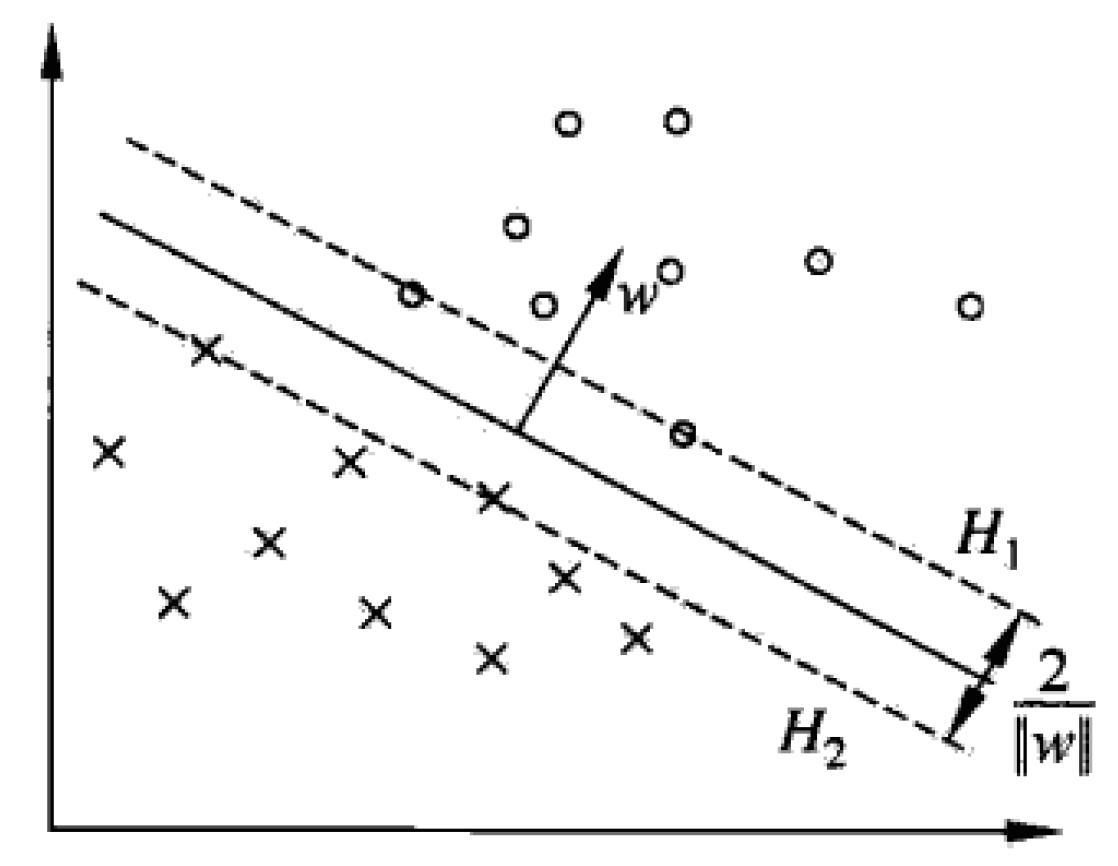
\includegraphics[width = 2in]{margin}
\end{figure}

Intuitively, the best separating hyperplane $H$ are only determined by those data points who are closest to $H$. Those data points are called {support vector}, and this method are called {support vector machine}.

Without loss of generality, we may restrict the norm of $\|w\|$ to be 1, which leads to a equivalent optimization problem
\begin{equation}
\max_{\|w\|_2 = 1} \min_{i} y_i(wx_i+b)
\end{equation}

Actually, {we can prove $\mathop{\rm argmax}_{\|w\|_2 = 1} \min_{i} y_i(wx_i+b)$ is nonempty, but here we just admit this fact and only prove the uniqueness of the solution.}

\begin{lemma}
	If $A_1,A_2$ are linearly separable, then
	\begin{equation}\label{binarySVM}
		\mathop{\rm argmax}_{\|w\|_2 = 1} \min_{i} y_i(wx_i+b)
	\end{equation}
	 is a singleton set.
\end{lemma}

\begin{proof}
	Denote $m(w,b) = \min_{i} y_i(wx_i+b)$. Notice that $m(w,b)$ is a concave homogeneous function w.r.t $w,b$ and $\|\cdot\|_2$ is a strictly convex norm. Suppose there are two solution $(w_1,b_1)$ and $(w_2,b_2)$ such that $w_1 \neq w_2$, take $\overline{w} = \frac{w_1 + w_2}{2}, \overline{b} = \frac{b_1 + b_2}{2}$, we must have
	\begin{equation}
		m(\overline{w},\overline{b}) \geq \frac{m(w_1,b_1)+ m(w_2,b_2)}{2} = \max_{\|w\|_2 = 1} m(w,b),
	\end{equation}
	and 
	\begin{equation}
		\|\overline{w}\|_2 < 1.
	\end{equation}
	So
	\begin{equation}
		m(\frac{\overline{w}}{\|\overline{w}\|_2},\frac{\overline{b}}{\|\overline{w}\|_2}) = \frac{m(\overline{w},\overline{b}) }{\|\overline{w}\|_2} > \max_{\|w\|_2 = 1} m(w,b),
	\end{equation}
	which leads to a contradiction. So all the solution must have the same $w$, we denote it as $w^*$. Then if $(w^*,b^*)$ is a solution of problem (\ref{binarySVM}), we must have
	\begin{equation}
		b^* \in \mathop{\rm argmax}_{b} m(w^*,b)
	\end{equation}
	Actually,
	\begin{equation}
		m(w^*,b) = \min\{b+\min_{x\in A_1} w^*x, -b +\min_{x\in A_2} (-w^*x)\},
	\end{equation}
	easy to observe that $\mathop{\rm argmax}_{b} m(w^*,b)$ is a singleton set and 
	\begin{equation}
		b^* = \frac{\min_{x\in A_2} (-w^*x) - \min_{x\in A_1} w^*x}{2}.
	\end{equation}
\end{proof}

Denote
\begin{equation}
	\theta^*_{SVM} = (w_{SVM}^*,b_{SVM}^*) = \mathop{\rm argmax}_{\|w\| = 1} \min_{i} y_i(wx_i+b).
\end{equation}


\subsection{Representation theorem and kernel methods}

\begin{theorem}[Representation Theorem]
	$w_{SVM}^*$ must be a linear combination of $x_i^T, i = 1,2,\cdots,N$.
\end{theorem}

\begin{proof}
	Denote
	\begin{equation}
		S = {\rm span} \{x_i^T\}_{i=1}^N
	\end{equation}
	Then we have
	\begin{equation}
		\mathbb{R}^{1\times d} = S \oplus^{\perp} S^{\perp}
	\end{equation}
	So $w_{SVM}^*$ can be uniquely decomposed as $w_{SVM}^* = w^*_S + w^*_{S^{\perp}}$ where $w_S\in S$ and $w^*_{S^{\perp}}\in S^{\perp}$. 
	We will prove that $w^*_{S^{\perp}} = 0$. Suppose not, we have
	\begin{equation}
		\|w^*_S\|_2 < \|w^*\|_2 = 1. 
	\end{equation}
	Notice that
	\begin{equation}
		w_{SVM}^* x_i = w_S^* x_i,\ \forall i = 1,2,\cdots,N.
	\end{equation}
	Thus we have
	\begin{equation}
		\min_{i} y_i(w_{SVM}^*x_i+b^*) = \min_{i} y_i(w_S^*x_i+b^*) 
	\end{equation}
	So
	\begin{equation}
	\min_{i} y_i(w_{SVM}^*x_i+b_{SVM}^*) < \frac{\min_{i} y_i(w_S^*x_i+b_{SVM}^*)}{\|w_S^*\|} = \min_{i} y_i(\frac{w^*_S}{\|w_S^*\|_2}x_i+\frac{b_{SVM}^*}{w^*_S}),
	\end{equation}
	which leads to a contradiction to the definition of $\theta_{SVM}^*$.
\end{proof}

We may rewrite the SVM problem as
\begin{align}{\label{SVM_Quadop}}
	\min_{w,b}&\ \|w\|^2,\\
	s.t.&\ y_i(wx_i+b) \geq 1,\ \forall i. 
\end{align}

We can simply prove that the solution of (\ref{SVM_Quadop}) is $\theta_{SVM}^*$ multiplies a positive scalar. So it still satisfies the representer theorem. Thus we can restrict $w$ to be in the set $S$. Assume that  
\begin{equation}
	w = \sum_{i = 1}^N \alpha_i x_i^T, 
\end{equation}
Denote $\alpha = (\alpha_1,\cdots,\alpha_N)^T$. We can rewrite the problem (\ref{SVM_Quadop}) as 
\begin{align}{\label{SVM_Quadop}}
\min_{w,b}&\ \alpha^T \big(<x_i,x_j>\big)_{N\times N} \alpha,\\
s.t.&\ y_i(\sum_{j = 1}^N <x_j,x_i>\alpha_j+b) \geq 1,\ \forall i. 
\end{align}
We can see that the whole problem is only determined by the inner product of data points but not the data itself directly. \\

Use the above formulation, we can induce nonlinearity in SVM. Denote the input space as $X$ where $\{x_i\}_{i=1}^N \subset X$. We use two steps to obtain a nonlinear classification model. First, we use a nonlinear feature mapping $\phi: X\rightarrow \mathcal{H}$ to map input space $X$ to a feature space $\mathcal{H}$. Second, we use linear SVM to do classification on $\{\phi(x_i)\}_{i=1}^N\subset \mathcal{H}$.\\

We may just asssume dataset after feature mapping $\phi$ is linearly separable. Then, the SVM problem after doing feature mapping can be formulated as
problem (\ref{SVM_Quadop}) as 
\begin{align}{\label{SVM_Quadop_innerprod}}
\min_{w,b}&\ \alpha^T \big(<\phi(x_i),\phi(x_j)>\big)_{N\times N} \alpha,\\
s.t.&\ y_i(\sum_{j = 1}^N <\phi(x_i),\phi(x_j)>\alpha_j+b) \geq 1,\ \forall i. 
\end{align}

Notice that to obtain the above problem we don't really need to know what exactly is the nonlinear mapping $\phi$, but only need to compute the value of $<\phi(x_i),\phi(x_j)>$. So we define a kernel function $k: X\times X\rightarrow \mathbb{R}$ such that 
\begin{equation}
	k(x,y) = <\phi(x),\phi(y)>,\ x,y\in X.
\end{equation}
Then the kernel SVM can be formulated as
\begin{align}{\label{SVM_Quadop_kernel}}
\min_{w,b}&\ \alpha^T \big(k(x_i,x_j)\big)_{N\times N} \alpha,\\
s.t.&\ y_i(\sum_{j = 1}^N k(x_i,x_j)\alpha_j+b) \geq 1,\ \forall i. 
\end{align}
In practice, we just need to find a proper kernel function instead of a good nonlinear feature mapping. Here we list some common used kernel functions:
\begin{itemize}
	\item Polynomial kernel: $k(x,y) = (a <x,y> + b)^n, a > 0, b\geq 0, n\in \mathbb{N}^+$.
	\item Gaussian kernel: $k(x,y) = e^{-\gamma\|x-y\|^2}, \gamma > 0$.
	\item Laplacian kernel: $k(x,y) = e^{-\gamma\|x-y\|}, \gamma > 0$
	\item Tanh kernel: $k(x,y) = \tanh(a<x,y>+b), a>0, b\geq 0.$
\end{itemize}

\subsection{Binary Logistic Regression}
For binary logistic regression, our score mapping can be written as
$\begin{pmatrix}
	\frac{1}{1+ e^{-(wx+b)}}\\
	\frac{1}{1+e^{wx+b}}
\end{pmatrix}$. \\
We can observe that, $(w,b)$ is classifiable if and only if
\begin{equation}
	\frac{1}{1+ e^{-y_i(wx+b)}} > \frac{1}{2},\ \forall i = 1,2\cdots,N.
\end{equation}

So we may consider to maximize following objetive
\begin{equation}
	P(\theta) = \prod_{i = 1}^N \frac{1}{1+ e^{-y_i(wx+b)}},\end{equation}
which is equivalent to minimize
\begin{equation}
L(\theta) = -\log P(\theta) = \sum_{i = 1}^N -\log(1+ e^{-y_i(wx+b)}),
\end{equation}

\begin{lemma}
	$L(\theta)$ is a strictly convex function without any global minima. 
\end{lemma}

To let the above problem have a global minima, we may add a $L_2$ regularization term as following
\begin{equation}
	\mathcal L(\theta,\lambda)  = L(\theta) + \lambda \|w\|_2^2 = \sum_{i = 1}^N -\log(1+ e^{-y_i(wx+b)}) + \lambda \|w\|_2^2,
\end{equation}

Actually, {we can prove $\mathop{\rm argmin}_{w,b} L(\theta,\lambda)$ is nonempty for $\lambda $ sufficiently small, but here we just admit this fact and only prove the uniqueness of the solution.}

\begin{lemma}
		If $A_1,A_2$ are linearly separable, then
	\begin{equation}\label{binaryLR}
	\mathop{\rm argmin}_{w,b} L(\theta,\lambda)
	\end{equation}
	is a singleton set for $\lambda $ sufficiently small.
\end{lemma}

\begin{proof}
Because $L(\theta)$ is strictly convex w.r.t. $\theta$ and $\|w\|^2$ is convex w.r.t. $\theta$, so $\mathcal L(\theta,\lambda)  = L(\theta) + \lambda \|w\|_2^2$ is stricly convex w.r.t. $\theta$, which implies our result directly.

\end{proof}

For $\lambda$ sufficiently small, denote
\begin{equation}
	\theta_{LR}(\lambda) = (w_{LR}(\lambda),b_{LR}(\lambda)) = \mathop{\rm argmin}_{w,b} L(\theta,\lambda).
\end{equation}


\begin{theorem}
	If $A_1,A_2$ are linearly separable, then $\frac{\theta_{LR}(\lambda)}{\|w_{LR}(\lambda)\|}$ converge to $\theta^*_{SVM}$ as $\lambda \rightarrow 0$, i.e.
	\begin{equation}
		\theta^*_{SVM} = \lim_{\lambda\rightarrow 0} \frac{\theta_{LR}(\lambda)}{\|w_{LR}(\lambda)\|}.
	\end{equation}
\end{theorem}